%% ---------------------------------------------------------------------------------------------------------------------

\chapter{Unsafe Security Problems}\label{ch:unsafe-security-problems}

This chapter presents an in-depth security analysis of possible consequences and vulnerabilities that can be caused by
misuses of the \unsafe{} \acrshort{API}.
It is organized into three main areas of danger.
First, buffer overflow bugs and their consequences including code injection and information leak vulnerabilities are
shown.
The following section is about incorrect conversion between slices and strings, which among others can lead to
\textit{use-after-free} bugs on multiple ways.
Finally, the dangers of conversions between types with architecture-dependent sizes are discussed.
Proof-of-concept code shows the practical exploitability of vulnerable implementations that contain incorrect usages of
\unsafe{} code, and threat models motivate the severeness and indicate how such a bug can be introduced in real-world
code, if the vulnerable code is not already taken from real open-source projects.

\begin{figure}[htp!]
    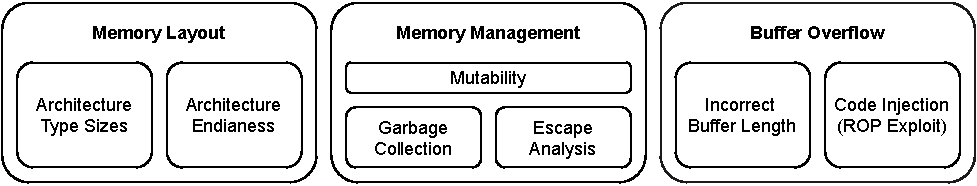
\includegraphics[width=\textwidth]{assets/figures/chapter3/outline3.pdf}
    \caption{Role of chapter 3 in the thesis outline}
    \label{fig:outline3}
\end{figure}



%% ---------------------------------------------------------------------------------------------------------------------

\section{Buffer Overflow Vulnerabilities}\label{sec:unsafe-security-problems:buffer-overflow}

The first main area of possible vulnerabilities in the context of the \unsafe{} \acrshort{API} are buffer overflows.
They are a rather common and dangerous problem with traditional systems programming languages like C, accounting for
many of the most severe security vulnerabilities~\cite{larochelle2001} \jl{second citation}.
Without the safety measures provided by the Go programming language to prevent them, as described in
Section~\ref{sec:background:memory-safety-layout}, which are not effective when using \unsafe{} code,
they can happen in Go just as well.


%% ---------------------------------------------------------------------------------------------------------------------

\subsection{Information Leak}\label{subsec:unsafe-security-problems:buffer-overflow:information-leak}

Go uses a strict type system that encodes the buffer length in the type information.
This prevents most buffer overflow vulnerabilities at compile time because the compiler can detect whether a given
buffer will be large enough to store the data that gets written to it, as described in
Section~\ref{sec:background:memory-safety-layout}.
However, this safety measure is circumvented when the \unsafe{} \acrshort{API} is used in Go.
Using direct casts through the \textit{unsafe.Pointer} type, it is possible to convert between buffers of different
sizes.
Listing~\ref{lst:information-leak} shows such a situation.

\begin{lstlisting}[language=Golang, label=lst:information-leak, caption=Buffer information leak proof of concept]
func main() {
    harmlessData := [4]byte{'A', 'A', 'A', 'A'}
    secret := [6]byte{'s', 'e', 'c', 'r', 'e', 't'}
    var leakingInformation = (*[10]byte)(unsafe.Pointer(&harmlessData[0]))
    fmt.Println(string((*leakingInformation)[:]))
}
\end{lstlisting}

In Line~4, a buffer of size four bytes called \textit{harmlessBuffer} is initialized with data.
Then, Line~5 declares a buffer containing a secret value, which should stay internal to the application.
Using the \unsafe{} \acrshort{API}, the \textit{harmlessBuffer} is then converted to a have a new length of ten bytes,
although there is no reallocation.
The resulting buffer is finally printed, which outputs not only the harmless four bytes, but also the secret.
The secret data could for example be a cryptographic private key or password information.
Therefore, this bug has created an information leak vulnerability.

To motivate a threat model that is more elaborated than this plain proof of concept,
Figure~\ref{fig:information-leak-threat-model-protocol} shows the specification of a simple client / server
communication protocol.
Both request and response types contain a version and message type field as well as a buffer for message-specific,
serialized data of length 512 bytes.

\begin{figure}[htp!]
    %\vspace{2mm}
    \centering
    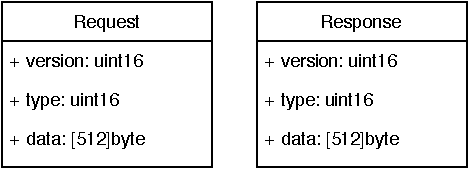
\includegraphics[width=0.5\textwidth]{assets/figures/chapter3/information-leak-threat-model-protocol.pdf}
    \caption{Example protocol to motivate threat model for unsafe cast}
    \label{fig:information-leak-threat-model-protocol}
    %\vspace{-10pt}
\end{figure}


If the client or server handling these messages uses the \unsafe{} \acrshort{API} to convert the serialized data to a
specific data structure, then the field lengths must match.
Imagine a company where two different teams are working on the client and server, respectively, and they printed the
protocol diagrams to hang them on the wall when the specification was decided.
A developer in one of the teams could easily miss the announcement of a protocol change that affects the buffer size,
and when they write incorrect code based on the outdated information on the printed diagram, the mistake could become
unnoticed in code review due to the same reason, a reviewer who looks at the protocol diagram in the team room.


%% ---------------------------------------------------------------------------------------------------------------------

\subsection{Code Flow Redirection}\label{subsec:unsafe-security-problems:buffer-overflow:code-flow-redirection}

To create a classic input-based buffer overflow vulnerability, we create a byte slice that has a length of 512 bytes,
but back it up with an underlying, much shorter byte buffer of only eight bytes.
As described in much more detail in Section~\ref{sec:unsafe-security-problems:slice-casts}, slices can be created using
a cast from the \textit{reflect.SliceHeader} type which reflects the internal slice representation.
This is done in Lines~8 to 10 of Listing~\ref{lst:buffer-overflow}.

\begin{lstlisting}[language=Golang, label=lst:buffer-overflow, caption=Buffer overflow leading to code flow redirection]
func main() {
    harmlessData := [8]byte{'A', 'A', 'A', 'A', 'A', 'A', 'A', 'A'}

    confusedSlice := make([]byte, 512)
    sliceHeader := (*reflect.SliceHeader)(unsafe.Pointer(&confusedSlice))
    sliceHeader.Data = uintptr(unsafe.Pointer(&(harmlessData[0])))

    _, _ = bufio.NewReader(os.Stdin).Read(confusedSlice)
}
\end{lstlisting}


Then, a reader is used to read input data into this malicious slice in Line~12.
Since it has a length of 512 bytes, the function reads up to this many bytes, however since the actual data array used
by the slice is much shorter, this will overflow into the memory behind the data array.
In this case, the \textit{harmlessData} array is created on the stack of the function, which means it is vulnerable to
buffer overflow exploits as described in Section~\ref{sec:background:memory-safety-layout}.
An attacker can use this vulnerability to redirect the code flow by carefully crafting the input data such that the
saved return instruction pointer on the stack is overwritten with the address of a function of the attacker's choosing.
To find the needed amount of padding before the address in the input data, as well as to find the target function's
address, the attacker can use a debugger such as \textit{GDB}.

A threat model for this kind of vulnerability would be an application that, similarly to the threat model described in
Section~\ref{subsec:unsafe-security-problems:buffer-overflow:information-leak}, uses a client server model, but this
time with a length information indicating how many bytes are sent within a variable-length data section as part of the
protocol.
If such a length field is used to construct a slice in the way shown in Listing~\ref{lst:buffer-overflow}, then an
attacker can control the resulting slice length and potentially exploit this bug to redirect to arbitrary code within
the binary.


%% ---------------------------------------------------------------------------------------------------------------------

\subsection{Code Injection using ROP}\label{subsec:unsafe-security-problems:buffer-overflow:code-injection}

Going a step further, this subsection shows how the same bug shown in the previous section in
Listing~\ref{lst:buffer-overflow} can be used with return-oriented programming (\acrshort{ROP}) to create a code
injection exploit.
The most basic approach to inject arbitrary code is to place machine instructions into the exploit input data, which
will then be written to the stack.
They can be before or after the address that gets overwritten at the position of the saved return instruction pointer,
but usually it is placed after because there is more space available.
The instruction pointer is then set to the start address of the machine instructions payload.
Since stack addresses can be slightly unpredictable in practice, for example because environment variables with
different lengths might be located on the stack, a \textit{NOP-slide} can be used to make the exploit more robust.
\textit{NOP}, or \textit{no-op}, is a machine instruction that does nothing at all, the processor simply continues with
the following instruction.
A \textit{NOP-slide} then is a series of such instructions.
Using this, it is sufficient to overwrite the return instruction pointer with an address somewhere within the
\textit{NOP} instructions to make the processor go through all remaining of them until it reaches the exploit code,
similar to sliding down a slope.
Thus, the address does not have to match the exact start of the payload code anymore, instead it can have a tolerance.
Figure~\ref{fig:stack-smashing-payload} shows a visualization of an example input data used to spawn a shell that an
attacker can then use to execute arbitrary code.

\begin{figure}[htp!]
    %\vspace{2mm}
    \centering
    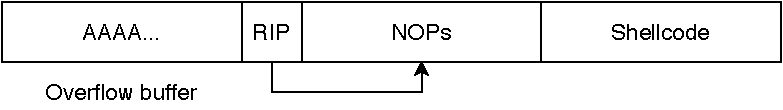
\includegraphics[width=0.8\textwidth]{assets/figures/chapter2/stack-smashing-payload.pdf}
    \caption{Stack smashing payload to inject exploit code}
    \label{fig:stack-smashing-payload}
    %\vspace{-10pt}
\end{figure}


However, such a type of exploit does not work an modern operating systems because they employ mitigation techniques
against this.
Executing machine instructions that are placed in memory that is part of the stack is prevented because the memory pages
containing the stack are marked as non-executable.
This technique is called Data Execution Prevention (\acrshort{DEP}).
It takes care of having sections in memory be either executable or writable, but not both.
That way, attackers can not easily write code into the memory and then jump into this code.
To work around \acrshort{DEP}, attackers can reuse existing functions in the binary, because as part of the text section
these are located on executable (but not writable) memory pages.
There is Address Space Layout Randomization (\acrshort{ASLR}), which loads dynamically-linked libraries into random
memory positions to avoid having predictable function addresses usable by attackers for code that is part of standard
libraries, like the C library \textit{glibc}.
However, \acrshort{ASLR} does not apply to statically-linked code, which the Go compiler mostly creates.
On top of that, the Go standard library is very large, providing a lot of reusable code fragments.

Return-oriented programming (\acrshort{ROP}) is a specific technique for reusing code that suggests jumping to very
small so-called gadgets, which are sequences of two or few more machine instructions that do not modify the stack
pointer register and end with a return instruction \jl{add citation}.
With these properties, gadgets can be chained because after the execution of a fragment the return instruction fetches
the next address to jump to from the stack, which the attacker can control.
Depending on the available \acrshort{ROP} gadgets, the attacker can therefore concatenate them and thus write a program
with a limited set of assembler instructions available.
The large Go standard library and its many available gadgets make exploiting a buffer overflow, once it exists in a Go
program, even easier compared to a C program where an attacker would have to work around \acrshort{ASLR}, for example.

A strategy to exploit a buffer overflow to achieve code injection using \acrshort{ROP} is to use the \textit{mprotect}
and \textit{read} system calls.
A system call, or syscall, is a function provided by the operating system which can be executed using the
\textit{syscall} machine instruction.
The processor registers control which syscall gets executed and which parameters it receives.
Therefore, an attacker only needs \acrshort{ROP} gadgets to control the contents of the registers, as well as to trigger
the syscall.
Using the \textit{mprotect} call, the attacker can set a memory area of their choosing to have both writable and
executable flags, for example the heap area.
Then, using the \textit{read} call, they can store data in that memory section, which is usually an exploit payload
spawning a shell to receive further arbitrary commands.
The payload is simply provided as part of the input string created by the attacker.
Finally, by using the address of the code area just like an address of another \acrshort{ROP} gadget the attacker can
make the processor jump to the payload code.
Because in contrast to the stack the code is now located on an executable page, it gets executed and the code injection
attack succeeds.
More details and proof-of-concept code for this type of exploit, as well as all other exploits presented in this
Chapter~\ref{ch:unsafe-security-problems}, are available in a dedicated repository on
\github{}\footnote{\url{https://github.com/jlauinger/go-unsafepointer-poc}}.


%% ---------------------------------------------------------------------------------------------------------------------

\section{Incorrect Slice and String Casts}\label{sec:unsafe-security-problems:slice-casts}

The second main area of danger with \unsafe{} usages is focused around the conversion of strings and slices of different
types.
Slices in Go are an array data type consisting of an underlying memory area and information about length and capacity.
The length indicates how many elements are currently contained in the slice, and the capacity denotes the allocated
space in memory.
When a subset of the slice is taken by specifying start and end indices, then a new slice is created that uses the same
underlying data array as the original one, and might have a capacity longer than its length if there are further
elements in the original slice after the end of the newly-taken subslice.
It is possible to increase the size of the new slice up to its capacity, but the size can never be larger than the
capacity.
When new elements are added to a slice using the \textit{append} function, then a new slice is created too which has a
higher length than the previous.
The runtime reuses the underlying data array of the original slice as well if its capacity is big enough, or allocates
a new array for the new slice if it is not.
Strings in Go are read-only \textit{[]byte} slices.
Usually they are encoded in UTF-8, but this is not required.
The length of a string is always the number of bytes needed to store its encoded form, which is often not the same as
the number of characters in the string.
It is important that strings are immutable because string literals are placed in a constant data section of the binary
when the code is compiled, meaning they are usually located within a read-only memory page and mutating them would cause
the program to receive a segmentation fault signal and crash.
Both slices and strings in Go are internally represented by a header structure that stores a pointer to the underlying
data array, as well as the size and capacity.
Listing~\ref{lst:reflect-header-types} shows the \acrshort{API} of these types.

\begin{lstlisting}[language=Golang, label=lst:reflect-header-types, caption=Reflect slice and string header types and API]
package reflect

type SliceHeader struct {
    Data uintptr
    Len int
    Cap int
}

type StringHeader struct {
    Data uintptr
    Len int
}
\end{lstlisting}

It is possible to access the internal structure of slices and strings by casting the slice to its header representation
using the \unsafe{} API.
Notice that the reference to the underlying data array has the type \textit{uintptr}, therefore it is not inherently
treated as a pointer type by the garbage collector (\acrshort{GC}).
Instead, there is a special case in the Go runtime that recognizes slices and strings and follows the address stored in
the \textit{Data} field to prevent it from getting collected.
As we will see in Section~\ref{subsec:unsafe-security-problems:slice-casts:gc-race}, there are however situations where
this fails.


%% ---------------------------------------------------------------------------------------------------------------------

\subsection{Incompatible Types}\label{subsec:unsafe-security-problems:slice-casts:incompatible-types}

Converting slices to strings and vice versa can be done simply by casting them, however this will cause the Go runtime
to allocate a new slice or string for the resulting value.
To improve efficiency by reusing the underlying data and only reinterpret it as data of a new type, it is possible to
use the \unsafe{} \acrshort{API} for an in-place cast.
Since the fields in the header structures shown in Listing~\ref{lst:reflect-header-types} are different in the presence
of the \textit{Cap} field, this is however only valid for conversions from slices to string.
In that case, the resulting string header, which shares the same location in memory with the original slice header, will
reuse the reference to the underlying data array as well as the length, and since the string header structure does not
contain any more fields the capacity information will simply follow unused in memory.

In contrast, when converting a string to a slice directly, the source header structure is too short.
The resulting slice header will use correct values for its data reference and length, but the capacity field will
contain whatever is located in memory directly after the original string header.
There is an instance of this incorrect cast in the \textit{k8s.io/apiserver} package that is part of the
\textit{Kubernetes} project, showing a conversoin from \textit{string} to \textit{[]byte}.
It is shown in Listing~\ref{lst:unsafe-string-to-bytes-direct}.

% k8s.io/apiserver/pkg/authentication/token/cache/cached\_token\_authenticator.go:235

\begin{lstlisting}[language=Golang, label=lst:unsafe-string-to-bytes-direct, caption=Incorrect direct cast between string and slice]
// toBytes performs unholy acts to avoid allocations
func toBytes(s string) []byte {
    return *(*[]byte)(unsafe.Pointer(&s))
}
\end{lstlisting}

The resulting slice with random data in its capacity field is dangerous to use.
Operations that read from a slice, like using it in a loop to iterate over its contents, mostly only use the data
reference and length.
However, any action on the slice that uses the capacity, like taking subslices from it or appending data, is undefined
and can therefore become a security vulnerability.


%% ---------------------------------------------------------------------------------------------------------------------

\subsection{Incorrect Length Information}\label{subsec:unsafe-security-problems:slice-casts:incorrect-length}

A second possible misuse in the context of slice conversions is an incorrect length value set in the slice header.
This can happen quickly if the length information is calculated dynamically, especially if the user-supplied input data
is used to deduce the resulting value.
An example of such a bug is shown in Listing~\ref{lst:go-fuse-bug}.
It is taken from the \textit{hanwen/go-fuse} library\footnote{\url{https://github.com/hanwen/go-fuse}}, a Go
implementation of the server specification used for the userspace filesystem (\acrshort{FUSE}) available for
Linux~\footnote{\url{https://www.kernel.org/doc/html/latest/filesystems/fuse.html}}.
We already submitted a patch for this bug to the authors, as described in more detail in
Section~\ref{sec:discussion:patches}.

% github.com/hanwen/go-fuse fuse/opcode.go:299

\begin{lstlisting}[language=Golang, label=lst:go-fuse-bug, caption=Incorrect slice length bug in the \textit{hanwen/go-fuse} library]
func doBatchForget(server *Server, req *request) {
    in := (*_BatchForgetIn)(req.inData)
    wantBytes := uintptr(in.Count) * unsafe.Sizeof(_ForgetOne{})

    if uintptr(len(req.arg)) < wantBytes {
        // We have no return value to complain, so log an error.
        log.Printf("Too few bytes for batch forget.",
                   len(req.arg), wantBytes, in.Count)
    }

    h := &reflect.SliceHeader{
        Data: uintptr(unsafe.Pointer(&req.arg[0])),
        Len:  int(in.Count),
        Cap:  int(in.Count),
    }
    forgets := *(*[]_ForgetOne)(unsafe.Pointer(h))
    // ...
}
\end{lstlisting}

\acrshort{FUSE} uses a client / server architecture where filesystem implementations present a server that handles
requests from a specific kernel module.
The kernel module acts like a regular filesystem driver, but instead of executing operations in kernel space, it
forwards them to the user space \acrshort{FUSE} server.
Communication is done through the \textit{/dev/fuse} device node.
The listing shows a part of the \textit{doBatchForget} function, which is used to clear files, identified by their inode
number, from a cache that the filesystem might have.
\textit{go-fuse} is designed in a way that incoming data from the \textit{/dev/fuse} node is passed to handler functions
as byte slices (\textit{req.inData} and \textit{req.arg}) containing the raw, serialized request.
The handler function then casts the data into a suitable structure to access individual fields.
In this case, the request is converted into an instance of the \textit{\_BatchForgetIn} type, which provides access to
the number of inodes to forget that are contained in the batch request through the \textit{in.Count} field.
The individual forget messages in serialized and concatenated form are available through the \textit{req.arg} array, so
to access them a new slice is created by defining its slice header from scratch.
In addition to the incorrect length calculation described in this section, this process of creating the slice has
multiple further problems which are described in the following Sections~\ref{subsec:unsafe-security-problems:slice-casts:gc-race}
and~\ref{subsec:unsafe-security-problems:slice-casts:escape-analysis}.
The created slice uses the incoming request data containing the forget messages (\textit{req.arg}) as its underlying
data array and the number of messages (\textit{in.Count}) both as length and capacity.

Since the \textit{in.Count} field is supplied as part of the request sent to the library, it can be controlled by an
attacker if they manage to conduct a man-in-the-middle (\acrshort{MITM}) attack and change the request for a malicious
one.
If the length is greater than the actual available number of data bytes, then the resulting \textit{forgets} slice will
read additional data after the end of the actual batch forgets request.
Depending of the concrete operation to forget inodes from a local cache, this could have severe consequences with
respect to security.
To prevent this from happening, the authors intended to check the length of the available data in Line~5, and if there
are too few bytes for the alleged number of forget requests, then the method should not proceed.
However, as the listing shows there is no actual code to stop further execution of the method, instead there is only a
log message noting that there was a malformed request with too few bytes available.
A proof-of-concept implementation of a potential attacker showed that the method actually reads invalid memory data
located after the request data.
In this case, a simple \textit{return} statement after Line~7 would have prevented this bug.

This example shows that small programming errors can lead to severe bugs and potential vulnerabilities when the
\unsafe{} \acrshort{API} is used.
The safety measures provided by Go are circumvented, thus a similar level of safety as in C is achieved.


%% ---------------------------------------------------------------------------------------------------------------------

\subsection{Implicit Read-Only}\label{subsec:unsafe-security-problems:slice-casts:read-only}

The conversion pattern shown in Listing~\ref{lst:string-to-bytes} is an \unsafe{} usage pattern that is used very
commonly in popular open-source projects, as the study described in Chapter~\ref{ch:go-geiger} revealed.

\begin{lstlisting}[language=Golang, label=lst:string-to-bytes, caption=Conversion from \textit{string} to \textit{[]byte} using \unsafe{}]
func StringToBytes(s string) []byte {
    strHeader := (*reflect.StringHeader)(unsafe.Pointer(&s))
    bytesHeader := reflect.SliceHeader{
        Data: strHeader.Data,
        Cap:  strHeader.Len,
        Len:  strHeader.Len,
    }
    return *(*[]byte)(unsafe.Pointer(&bytesHeader))
}
\end{lstlisting}

It takes a string argument and converts it into a slice of bytes without allocating additional memory.
This allows to access the raw bytes contained in the string in an efficient manner.
First, the string is converted into the \textit{reflect.StringHeader} representation.
Then, a slice header is created as a composite literal and the reference to the underlying data array and length
information are copied from the string header.
The capacity is set to the same value as the length, as it would be in a slice that uses the full allocated capacity.
Finally, the slice header is converted into an actual \textit{[]byte} slice which is returned.

There are three not obvious but very dangerous problems that come with this type of slice creation, which are described
in this and the following two subsections.
The first is that the resulting slice is implicitly read-only.

Regularly, slices in Go are mutable and strings are not.
The reason for this is that slices are created dynamically, with their backing array usually placed on the heap, while
strings are mostly constants that are part of the constant data or text section of the program binary after compilation.
The actual string characters, to which the data reference in the string header will be pointing, are therefore usually
located on a memory page that is not writable, and mutating the string would thus make the program receive a
segmentation fault signal from the operating system.
To statically prevent this at compilation time, strings are always immutable in Go, while slices are mutable.
If a developer writes code that changes parts of a string in-place, then the compiler will not accept the code and thus
prevent the possible segmentation fault.

In contrast, slices are mutable, and thus so is the slice returned by the \textit{StringToBytes} function in
Listing~\ref{lst:string-to-bytes}.
Code that changes the resulting slice will be accepted by the compiler because it is not able to infer its connection to
a former string.
However, since the slice uses the same underlying data array as the original string used to do, the data is still
potentially located within read-only memory, and modifying it will crash the program.
It is only implicitly read-only, but the runtime is not aware of it.
While this first problem of the conversion pattern does not cause a direct security vulnerability, it underlines that
there are many consequences of using the \unsafe{} \acrshort{API} that are not obvious.
Although it is possible in theory to manually ensure that no usages of the \textit{StringToBytes} function modify the
slice it returns, in practice it is very hard to do so, especially if new developers join the project after time and
start using the function without having all possible consequences in mind.


%% ---------------------------------------------------------------------------------------------------------------------

\subsection{GC Race Use-After-Free}\label{subsec:unsafe-security-problems:slice-casts:gc-race}

The second problem caused by the conversion shown in Listing~\ref{lst:string-to-bytes} is a \textit{use-after-free} bug
caused by a race condition involving the garbage collector (\acrshort{GC}) used by Go.
Go uses a move-and-sweep GC that runs concurrently with all other threads of a program to free unused heap
memory~\cite{sibiryov2017}.
It is triggered by one of two conditions, either when the heap usage has increased to a specific size (usually when the
usage has doubles since the last \acrshort{GC} run), or after a fixed time has passed without any \acrshort{GC} runs.
The \acrshort{GC} takes all variables that are present in the scope of the program and marks them as live.
Then, it recursively follows all pointer types within live variables and marks their target values as live, too.
After this marking phase has completed, the sweep phase frees all memory that is not marked as live.
Finally, the markings are reset and a new \acrshort{GC} run can be triggered.

Figure~\ref{fig:gc-visualization} shows a visualization of the marking phase in a \acrshort{GC} run.
The variables in scope can be either on the stack, which is not managed by the \acrshort{GC}, or on the heap, in which
case they are marked as being live as well.
The arrows indicate references from pointer types to their targets, and the blue values on the heap are the ones marked
as live.
The white heap values will be freed in the sweep phase of the \acrshort{GC}.

\begin{figure}[htp!]
    %\vspace{2mm}
    \centering
    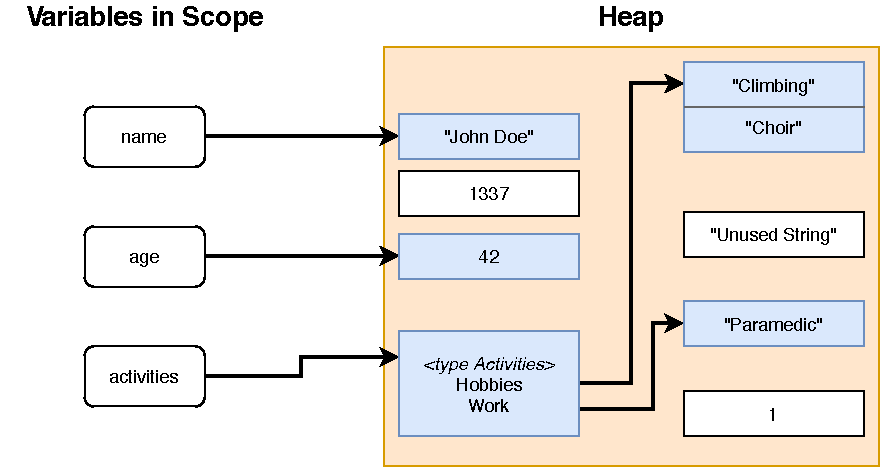
\includegraphics[width=0.6\textwidth]{assets/figures/chapter3/gc-visualization.pdf}
    \caption{Garbage Collector Visualization}
    \label{fig:gc-visualization}
    %\vspace{-10pt}
\end{figure}


The \acrshort{GC} treats all pointer types and the special \textit{Data} field of actual slices and strings as reference
types.
Importantly though, it does not treat normal \textit{uintptr} values as references although they contain addresses.
This means that converting a \textit{uintptr} value to an \textit{unsafe.Pointer} value is an invalid and dangerous
operation.
If the \textit{GC} runs while the pointer has not been constructed, then it does not mark the value at the address
stored in the \textit{uintptr} value as live and thus frees the memory.
Creating an \textit{unsafe.Pointer} from this address therefore creates a potentially dangling pointer because it points
to memory that has been freed.
This is a \textit{use-after-free} bug.

The conversion pattern between strings and slices shown in Listing~\ref{lst:string-to-bytes} contains exactly this bug.
The \textit{Data} field of the \textit{reflect.SliceHeader} structure created in Line~3 is of type \textit{uintptr}, and
since the header value is not derived by cast from a real slice it does not benefit from the special case built into the
Go runtime that treats \textit{uintptr} references that are part of slice and strings as references, too.
Specifically, the problem is that the slice header has been constructed as a composite literal.
Therefore, after Line~7 the \textit{bytesHeader} variable effectively becomes a plain \textit{uintptr} value, and the
original string \textit{s} is not used any longer.
However, at this point there is no real slice created yet as this happens net earlier than in Line~8.
The underlying data array of the string \textit{s} is therefore not a live value as far as the \acrshort{GC} is
concerned.

\begin{figure}[!t]
    \vspace{2mm}
    \centering
    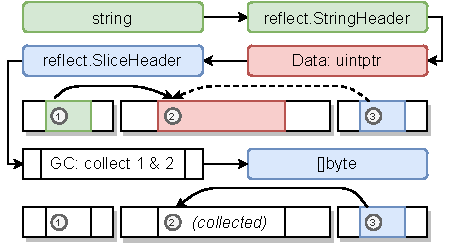
\includegraphics[width=0.4\textwidth]{gfx/figures/gcrace-vuln.pdf}
    %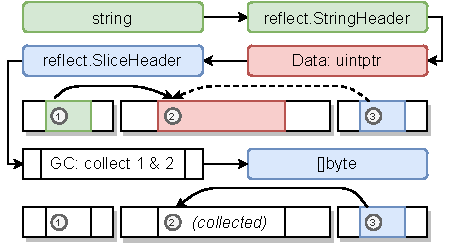
\includegraphics[width=0.48\textwidth]{gfx/figures/gcrace-vuln.pdf}
    \caption{GC race and escape analysis flaw}
    \label{fig:gcrace-vuln}
    \vspace{-8pt}
\end{figure}


If the \acrshort{GC} runs at the wrong time, the underlying data array used in the slice might have already been
collected by the time the resulting slice is created.
This is possible because since the \acrshort{GC} runs concurrently to the application logic, it can trigger at any time.
This is especially true if the Go program has several threads that all contribute to the heap usage.
Figure~\ref{fig:gcrace-vuln} illustrates the vulnerability.
The green boxes show the original string value and its header, which is represented at position 1 in the memory schema.
The reference to the underlying data of the string and resulting slice is shown in red at memory position 2.
Then the slice header is created, which is colored blue and located at position 3 in the memory.
References indicated by arrows are strong if the arrow is continuous, like the reference the string header has, and
weak if the arrow is dashed, like the new slice header has.
Then, after the \textit{GC} runs, there is only the resulting bytes slice left, which is also shown in blue.
It now has a strong reference to the underlying data array (at position 2), but since the \acrshort{GC} has already run
while there was only a weak reference to it, the data has been collected.
The resulting bytes slice is now a dangling pointer into the former string data in memory, and the
\textit{use-after-free} bug is complete.

A common variation to this insecure casting pattern is to omit storing the slice header that is created as a composite
literal in a variable and instead casting it into the resulting slice value within the same statement, as is shown in
Listing~\ref{lst:string-to-bytes-1statement}.

\begin{lstlisting}[language=Golang, label=lst:string-to-bytes-1statement, caption=Unsafe slice cast in one single statement]
strHeader := (*reflect.StringHeader)(unsafe.Pointer(&s))
return *(*[]byte)(unsafe.Pointer(&reflect.SliceHeader{
    Data: strHeader.Data,
    Cap:  strHeader.Len,
    Len:  strHeader.Len,
}))
\end{lstlisting}

This does however not affect the bugs and vulnerabilities shown in this
Section~\ref{sec:unsafe-security-problems:slice-casts}.
In fact, the assembly that the code gets compiled to is exactly the same for both versions in
Listings~\ref{lst:string-to-bytes} and~\ref{lst:string-to-bytes-1statement}.
Even if the assembly would be different, performing the creation of a slice header as a composite literal and casting it
to an actual slice in the same statement would still not avoid creating a plain \textit{uintptr} reference to the
underlying data array as far as the \acrshort{GC} is concerned.
This is because the \acrshort{GC} concurrency is at the level of machine instructions, not statements in the Go source
code.


%% ---------------------------------------------------------------------------------------------------------------------

\subsection{Escape Analysis Use-After-Free}\label{subsec:unsafe-security-problems:slice-casts:escape-analysis}

A third problem that comes with the incorrect construction of a new slice shown in Listing~\ref{lst:string-to-bytes} in
the previous section is that the Go compiler's escape analysis (\acrshort{EA}) algorithm fails.
\acrshort{EA} is used to decide whether a variable can be placed on a function's stack or needs to be allocated on the
heap.
The stack is preferred because there is no explicit deallocation step needed to free the stack memory, instead the stack
frame is removed completely when the function returns as described in Section~\ref{sec:background:memory-safety-layout}.
In \acrshort{EA}, a value is said to escape if references to it can live longer than the current function's lifetime.
If it does escape, then it needs to be allocated on the heap so that when the function has terminated, references that
still exist can continue to access the memory even though the function stack has vanished.
Otherwise, it can be placed on the stack.
The \acrshort{EA} analysis employed by the Go compiler works by checking for each variable that is declared in a
function whether a reference to it is stored in another value or passed to another function.
If there is a reference stored in another object, this object has to be checked too, and if it escapes then so does the
original variable.
The same is true for functions: if the variable gets passed to another function then the \acrshort{EA} algorithm
transitively looks into that function and determines if the value escapes there.
If it does, then it must also be treated as an escaped value in the original function.
Finally, if the function returns a reference to the variable then it obviously escapes as well.

The insecure string to slice conversion shown in Listing~\ref{lst:string-to-bytes} breaks the \acrshort{EA}.
This is because for a similar reason to the \acrshort{GC}, it misses the connection between the string parameter and
the slice return value.
Listing~\ref{lst:escape-analysis-flaw} shows a proof of concept of this problem.

\begin{lstlisting}[float=tp, language=Golang, label=lst:escape-analysis-flaw, caption=Escape analysis flaw proof of concept]
func main() {
    bytesResult := GetBytes()
    // expected stdout is "abcdefgh"
    // actual output is random invalid data
    fmt.Printf("main: %s\n", bytesResult)
}

func GetBytes() []byte {
    reader := bufio.NewReader(strings.NewReader("abcdefgh"))
    s, _ := reader.ReadString('\n')
    out := StringToBytes(s)
    // expected stdout is "abcdefgh"
    // actual output is "abcdefgh"
    fmt.Printf("GetBytes: %s\n", out)
    return out
}
\end{lstlisting}

In the function \textit{GetBytes}, a string variable \textit{s} is created by reading a string through a buffered
reader.
It is necessary to use the reader instead of a string literal, because with a literal the effects of the vulnerability
would not be visible.
This is however no restriction to the proof of concept.
Creating the string from a reader is similar to accepting dynamic user input.
Next, the string is converted to a byte slice using the insecure \textit{StringToBytes} function in Line~10.
Printing the resulting slice in Line~12 then yields the expected output equal to the original string, which is
\textit{abcdefgh}.
Finally, the slice is returned to the caller function, which in this case is the \textit{main} function in Line~2.
The slice is printed again in the \textit{main} function in Line~4, and while the expected output would be identical,
this time invalid, random data is printed.

The reason for this is that when the Go \acrshort{EA} algorithm determines where to allocate the string \textit{s} in
the \textit{GetBytes} function, it sees that \textit{s} is passed to the \textit{StringToBytes} function and therefore
transitively analyzes that function.
Within that function, \textit{s} is used in a cast to the \textit{strHeader} variable in Line~2 of
Listing~\ref{lst:string-to-bytes}, then that is used to construct the \textit{bytesHeader} variable, but at this point
there no further references to the underlying data array of \textit{s} because both \textit{s} and
\textit{strHeader} are not used further in the function.
Similarly to the \acrshort{GC} mark algorithm, the \textit{Data uintptr} field would only be treated as a reference with
respect to escape analysis if the slice header had been created by cast from an actual slice.
Therefore, the \acrshort{EA} determines that \textit{s} does not escape in \textit{StringToBytes}, and since it is not
used any longer in \textit{GetBytes}, it does not escape at all and is placed on the stack of the \textit{GetBytes}
function.
The \textit{EA} algorithm fails to detect that there is a reference to parts of the string \textit{s} stored in the
\textit{out} variable, which obviously escapes as it is returned.

Printing the \textit{out} slice in Line~13 works because the stack of the \textit{GetBytes} function is still there at
this point.
However, when the function returns the stack frame is removed, and thus \textit{bytesResult} in Line~2 has become a
dangling pointer into the former stack of \textit{GetBytes}.
This is a \textit{use-after-free} bug because that memory can and probably will be reused at that point.
The print statement in Line~4 outputs invalid data for this reason.
If the \textit{main} function would modify the contents of the \textit{bytesResult} slice, it would change arbitrary
memory, with possible consequences such as information leaks or code injection.


%% ---------------------------------------------------------------------------------------------------------------------

\section{Architecture-Dependent Types}\label{sec:unsafe-security-problems:architecture-dependent-types}

The third area of possible vulnerabilities concerns types that have a different size or alignment on different
architectures.
A feature of Go is portability between different platforms.
The same source code can usually be compiled for many different architectures without any changes in its behavior.
However, this is only true as long as the \unsafe{} \acrshort{API} is not used.
Since \unsafe{} code allows direct conversion between arbitrary types, there can be inconsistencies between the sizes
and alignments of structure fields on different architectures.
An example of this is shown in Listing~\ref{lst:architecture-dependent-types-cast}.

\begin{lstlisting}[language=Golang, label=lst:architecture-dependent-types-cast, caption=Incorrect cast between architecture-dependent types]
func main() {
    bytesResult := GetBytes()
    fmt.Printf("main: \%s\n", bytesResult) // expected (but failed) stdout is "abcdefgh
}

func GetBytes() []byte {
    reader := bufio.NewReader(strings.NewReader("abcdefgh"))
    s, _ := reader.ReadString('\n')
    out := StringToBytes(s)
    fmt.Printf("GetBytes: \%s\n", out) // expected stdout is "abcdefgh"
    return out
}
\end{lstlisting}

There are two structure types declared, \textit{PinkStruct} and \textit{VioletStruct}, both of which have two fields
\textit{A} and \textit{B}.
While field \textit{B} has the same type (\textit{uint8}) in both types, field \textit{A} is of type \textit{int} and
\textit{int64}, respectively.
An instance of \textit{PinkStruct} is created in Line~11, which is then converted to \textit{VioletStruct} in Line~12.
This is however only a valid operation if \textit{int} and \textit{int64} share the same size and alignment.

This is true only for 64-bit platforms like \textit{amd64}.
If the code is run on such an architecture, the conversion works fine and the field values in the resulting variable
\textit{violet} are as expected.
In contrast, if the code is run on an architecture where \textit{int} and \textit{int64} have different size or
alignment, then the values of \textit{violet} are undefined.
This is the case for example when the code is run on a 32-bit platform like \textit{i386}.
When the structure definitions are not placed directly next to each other but in separate files, packages, or even
modules, then spotting the difference between the incompatible structs is much harder.
On top of that, the bug might never occur in testing but only on specific platforms that get used in production.
Possible consequences of a bug like this depend on how the resulting struct is used in the remainder of the program.
If data gets written to it, it changes invalid memory which can lead to a code injection vulnerability, and if it is
passed as output it could create an information leak vulnerability.
